\chapter{Proposed Methodology}

The proposed virtual assistant system is designed to streamline various tasks within a banking application, significantly enhancing efficiency and user experience. In the banking sector, employees often spend considerable time manually processing transactions and handling customer requests, which can be tedious and time-consuming. Our virtual assistant can drastically reduce this time. The system employs a large language model (LLM) to understand user queries and generate appropriate functions. These functions are then executed by an action engine, which processes the results and returns them in a JSON format. The results are subsequently displayed to the user in an easily understandable manner, making banking operations faster and more efficient. This transformation can decrease task completion time from several hours to mere minutes, thereby significantly improving productivity.

\vspace{1.5mm}

\begin{figure}[h!]
    \centering
    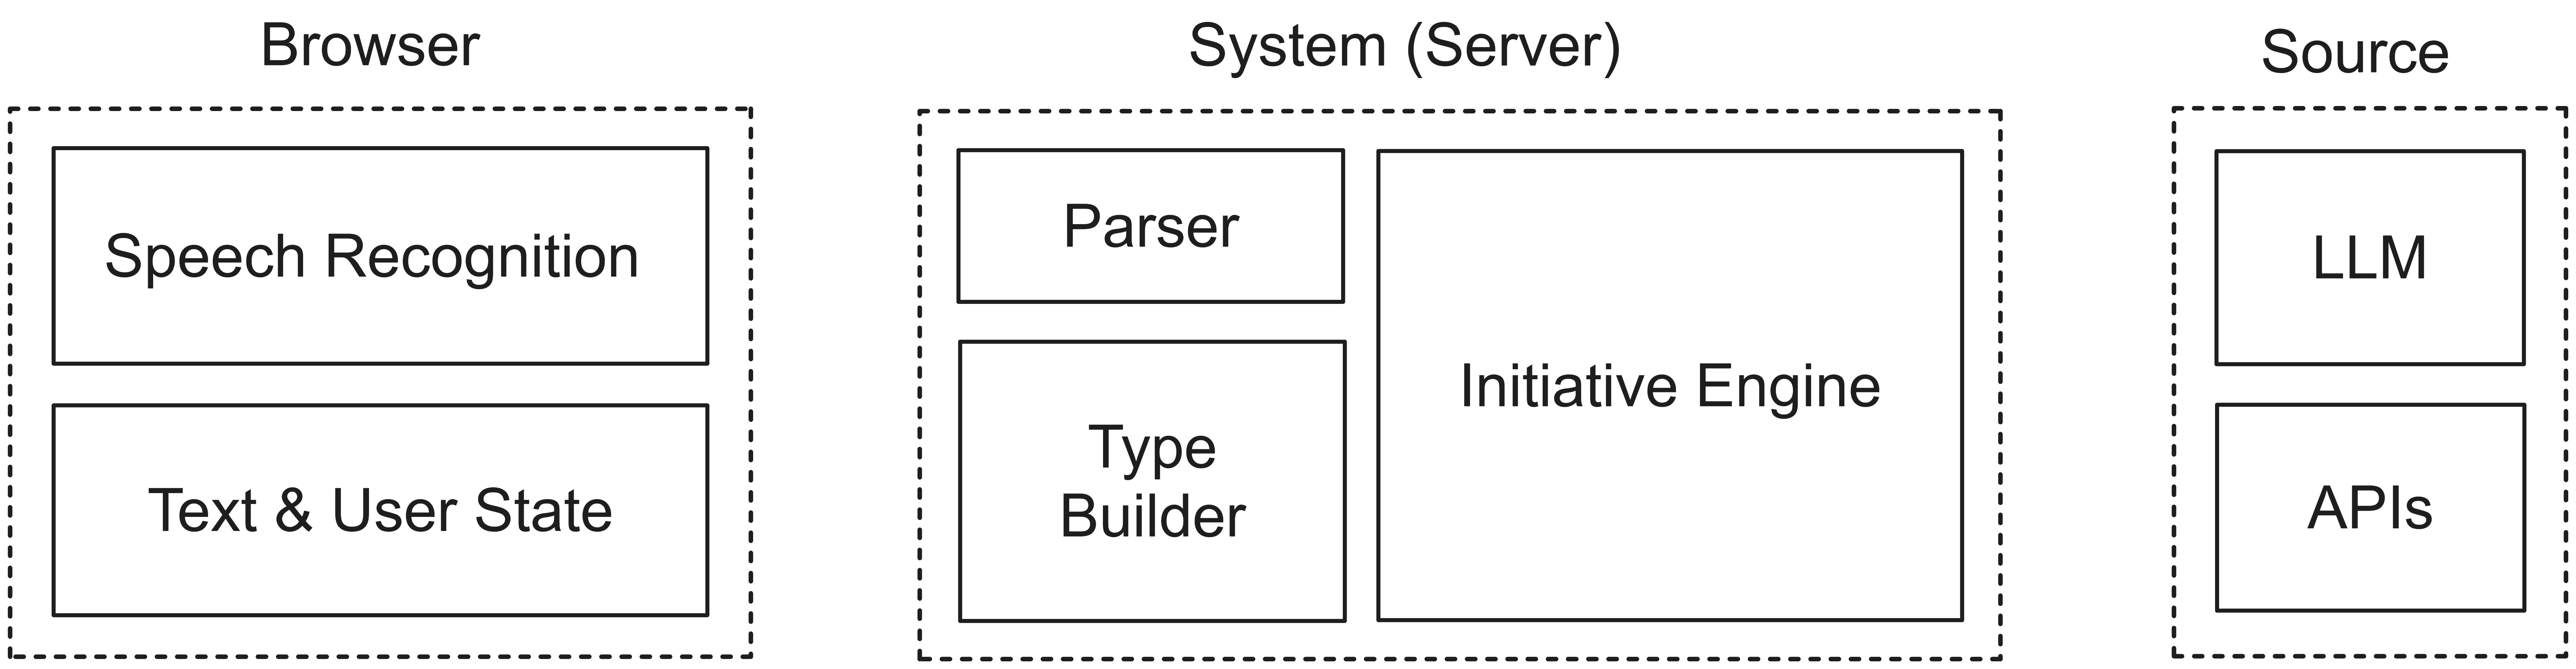
\includegraphics[width=0.9\textwidth]{Images/lit_review/main_components.png}
    \caption{Main components of the system}
\end{figure}

\clearpage

\noindent
As per the overall literature survey and research, it is evident that the modular approach for system building is the best. A modular design for the system is illustrated using Figure 3.1, where the idea of modules would be the building blocks for the system and they serve the purpose of ease of development and modification. The explanation for each block is as follows: 

\begin{enumerate}
    \item Browser: Users end of the system that supports Voice and Text input commands. Also keep track of user state on application.
    \item System: Server side of the application that handles parsing of I/O and enable chained execution of APIs.
    \item Source: Source and definitions of third party APIs. Language Model that enables the system to understand user commands.
\end{enumerate}.

\section{Overview of the Proposed System}

\noindent The core objective of this project is to create a highly intuitive and developer-friendly library that help developers to build their own Action Models on top of any Large Language Model. By employing LLM as the base source of knowledge and language understanding, the library allows developers to define third party APIs or function definitions for the Action Model. The captured user command (voice) are processed to pure text string within browser and passed to server. The server is already equipped with core function definitions and parsing libraries to ensure precise and reliable conversion of data type, argument type and return type to pure string that can understandable by LLM. The LLM is also instructed to respond with JSON format data, which is then processed by the server to execute the function and return the result in JSON format. The result is then passed to the browser and displayed to the user.

\noindent This process ensures a seamless and efficient user experience with the application or software. Eventually offering developers and software business owners a better user experience feedback. With the integration of LLM and LAM (Large Action Model) technologies, this applications not only enhances the speed and efficiency of extracting data but also paves the way for Automated function calling tools.

\begin{figure}[htbp]
  \centering
  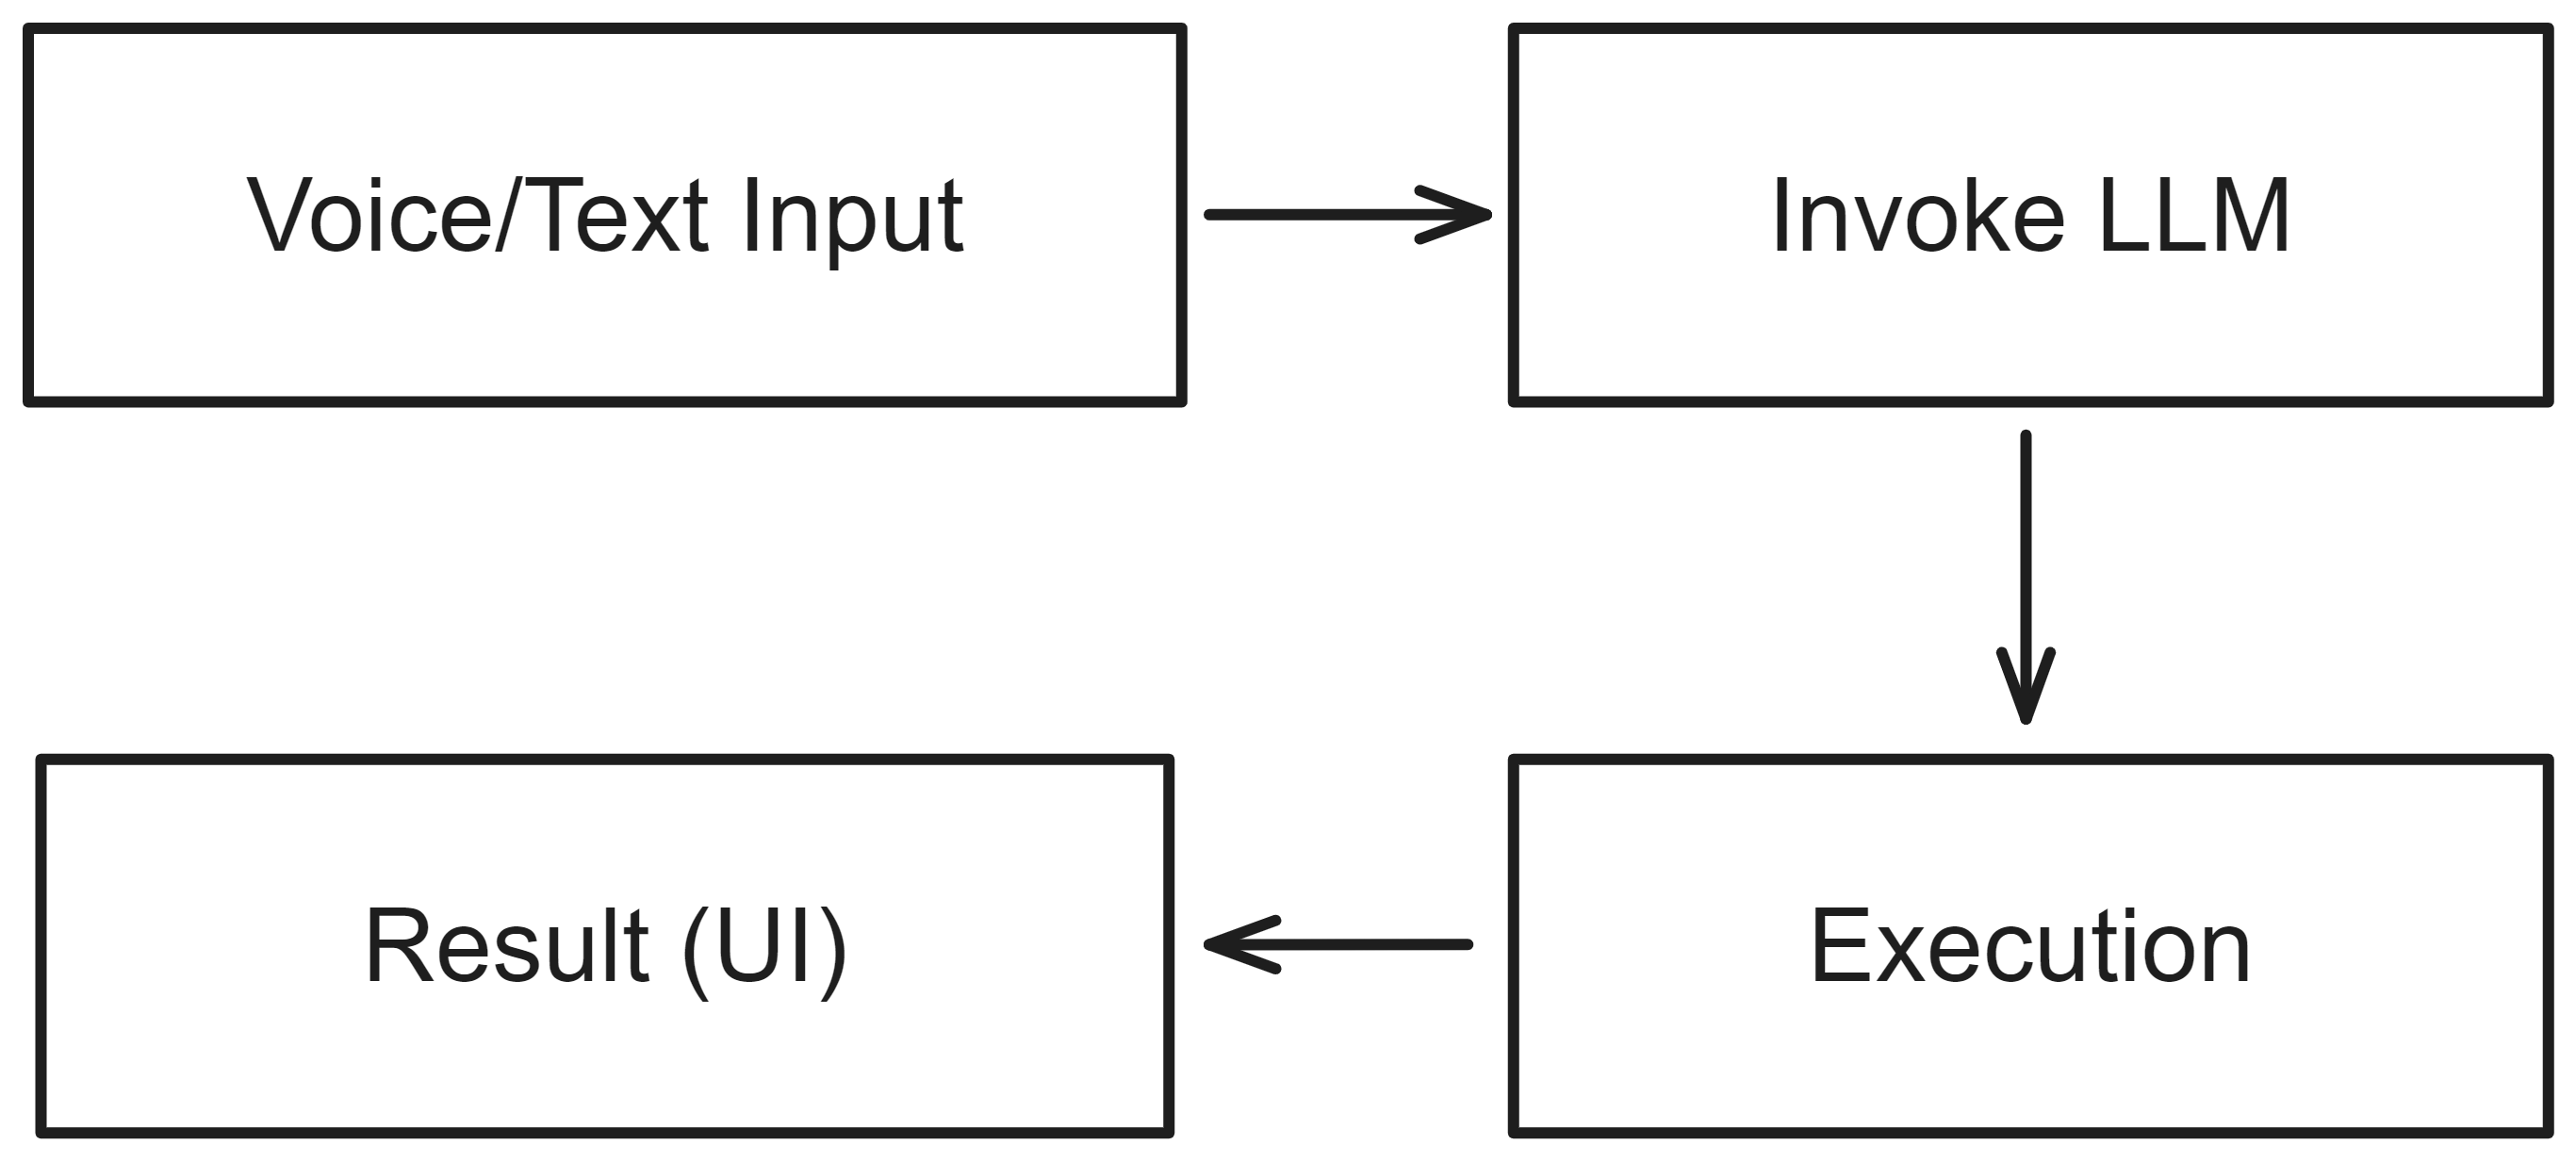
\includegraphics[width=0.7\textwidth]{Images/prop_sys/overview_prop_sys.png}
  \caption{Overview of proposed system}
\end{figure}

\clearpage

\section{Detailed Description Of The System}

\noindent
The application features a professional and minimal user interface, developed using NextJS and TypeScript. Designed to enhance interactivity and easiness, this interface serves as the entry point for users to interact with the banking applications we built seamlessly. A input box and voice icon in the center enables users to quickly open the access to input their requirements. This intuitive design fosters a professional environment, empowering users with a streamlined approach to their tasks.

\noindent The input text/voice is processed by the inbuilt browser voice API and sended to server. Figure 3.3 shows the recognized table structure.

\begin{figure}[h!]
    \centering
    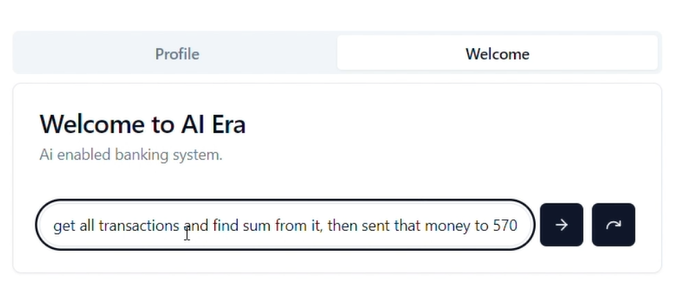
\includegraphics[width=0.8\textwidth]{Images/prop_sys/ui_for_bank_app.png}
    \caption{UI for simple banking application}
\end{figure}

\noindent \textbf{The server is the implementation of this Action Model with LLM and supports for function calling APIs.} The server is built with NextJS with tRPC, DrizzleORM and Supabase. These are incredible and popular new technologies used for building Full Stack Applications. NextJS enables server side web applications with ReactJS. tRPC is for APIs. Supabase is a Postgres Database provider and DrizzleORM help to connect the database.\\ 

\noindent The input command from client side is processed with \textbf{custom library we build called Initiative} will combain with type definitions extracted from available functions provided, which help the LLM to understand the environment around it. For this banking application, input of user command with the user state inside the application is combained with type definitions of functions or third party APIs available and passed to LLM. Then the LLM is instructed to respond in JSON format of "what should do next?". Instructions from LLM is parsed and reconstructed to executable list of functions. This list passed to execution engine with user permission of each functions. The engine execute the function with corresponding parameters from LLM and result is returned back to client as UI.

% \noindent For extracting cells from the image and converting the extracted cells to its digital text, the model makes use of the img2table library and an OCR engine respectively, and for executing the whole process, there are two methods: one involves the use of \textbf{img2table library}, and the other involves \textbf{extracting cell coordinates}. A detailed explanation and side-by-side comparison are written in paragraphs and with a comparison Table 3.1 respectively.\\

% \noindent Method 1: \textbf{img2table library}\\

% \noindent In this method, the system uses the img2table library in combination with PaddleOCR (built-in to the same library) to detect the table, extract coordinates of table cells, and perform OCR on each extracted cell using PaddleOCR. These three processes are executed using an attribute called on the input image, which is converted to the proprietary document type of the library.\\

% \begin{figure}[h!]
%   \centering
%   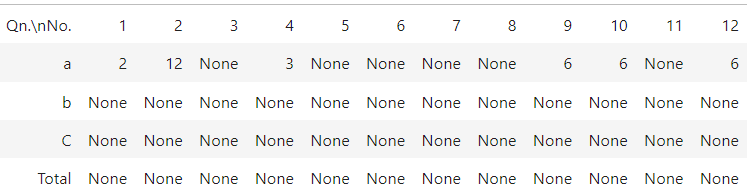
\includegraphics[width=0.8\textwidth]{Images/prop_sys/paddle_ocr_output.png}
%   \caption{DataFrame Output of img2table library method using PaddleOCR}
% \end{figure}


% \begin{table}[ht]
%   \centering
%   \footnotesize
%   \begin{tabular}{|c|c|c|c|c|c|c|c|c|c|c|c|c|}
%   \hline
%   Qn. No. & 1 & 2 & 3 & 4 & 5 & 6 & 7 & 8 & 9 & 10 & 11 & 12 \\
%   \hline
%   a & 2 & 12 & None & 3 & None & None & None & None & 6 & 6 & None & 6 \\
%   \hline
%   b & None & None & None & None & None & None & None & None & None & None & None & None \\
%   \hline
%   c & None & None & None & None & None & None & None & None & None & None & None & None \\
%   \hline
%   Total & None & None & None & None & None & None & None & None & None & None & None & None \\
%   \hline
%   \end{tabular}
%   \caption{DataFrame output of img2table library method using PaddleOCR}
% \end{table}


% \noindent  Consequently, the programmer does not have explicit control over the individual stages to meet specific requirements. The resulting DataFrame (shown in Table 3.1) is then post-processed to remove the first column and the first and last rows.\\

% % \vspace{1.5mm}

% \noindent Method 2: \textbf{Cell Coordinates Extraction}

% \vspace{1mm}

% \noindent In this method, the system extracts only the cell coordinates using the img2table library. The extracted table cells are stored in an ordered dictionary.

% \vspace{1mm}

% \noindent \textit{OrderedDict is a dictionary subclass in Python that maintains the order of key-value pairs. Even if the value of a key is modified, the order of the keys remains unchanged. In contrast, a regular dictionary does not guarantee a specific order and may reorder the keys when their values are modified.}

% \vspace{0.5mm}

% \noindent In the ordered dictionary data structure, each key represents a single row of the mark table, so deleting a key is equivalent to removing a row from the table, thus deleting the first and last keys of the ordered dictionary. There is a  need to remove the first column (column with A, B, and C written) also, but it could be easily done after converting the presently existing cells to their DataFrame format.

% \noindent From the two methods above, the second method was chosen as it has the following benefits (shown in Table 3.2).

% \begin{table}[h!]
%   \centering
%   \renewcommand{\arraystretch}{1.2}
%   \begin{tabular}{|l|p{4.5cm}|p{4.5cm}|}
%       \hline
%       \textbf{ } & \textbf{Cell Coordinates Extraction Method} & \textbf{PaddleOCR Method} \\
%       \hline
%       \textbf{Speed} & Very fast as it works with built-in data structures. & Slow, as it runs the big PaddleOCR engine. \\
%       \hline
%       \textbf{Programmer's Control} & Highly controllable & No control \\
%       \hline
%       \textbf{Ease of programming} & Difficult & Easy \\
%       \hline
%       \textbf{Ease of understanding} & Medium & Easy Outwards, Internal working codes are complex.\\
%       \hline
%       \textbf{Time taken} & 13 seconds for 5 papers & 44 seconds for 5 papers \\
%       \hline
%   \end{tabular}
%   \caption{Comparison of Table Processing Methods}
% \end{table}

% \clearpage

% \noindent Once the ordered dictionary is processed, the remaining table cells are cropped based on these coordinates and forwarded to the CNN model. Table 3.3 depicts the classification time taken by the CNN model for each individual image, showcasing the exceptional speed and efficiency of the model. The CNN model is specifically designed with a minimum number of layers to make it perform efficiently on smaller images. This way, it ensures that the proposed system prioritizes speed without compromising accuracy. It boasts an impressive capability to process five images in a mere 13 seconds, showcasing its remarkable performance.

% \begin{table}[htbp]
%     \centering
%     \begin{tabular}{|c|c|}
%         \hline
%         Image Count & Time per step (ms) \\
%         \hline
%         1 & 23 \\
%         2 & 18 \\
%         3 & 17 \\
%         4 & 17 \\
%         5 & 16 \\
%         6 & 16 \\
%         7 & 16 \\
%         8 & 23 \\
%         9 & 20 \\
%         10 & 19 \\
%         \hline
%         Average time: & 18.5 \\
%         \hline
%     \end{tabular}
%     \caption{Classification time taken for CNN OCR Model Version 1}
% \end{table}

% \noindent The output after the classification and some processing is a DataFrame. This DataFrame is post-processed to remove the first column using a \textit{Pandas} function.\\

% \noindent The final dataframe will be converted to a NumPy array for flattening the DataFrame; And the two-dimensional array is flattened column-wise to get the marks corresponding to each sub-division (1A, 1B, ..., 12B, 12C). The output is a one-dimensional array that represents the marks scored by a student in individual questions.

% \clearpage

% \noindent The flattened array is incorporated into a dictionary to store the marks of individual students. Following this step, additional coding is applied for post-processing, which includes the removal of columns with identical entries and adding the columns \textit{Roll No.} and \textit{Name} to the left side of the DataFrame. This DataFrame is then converted to CSV format without the index values.\\

% % \begin{figure}[h!]
% %     \centering
% % {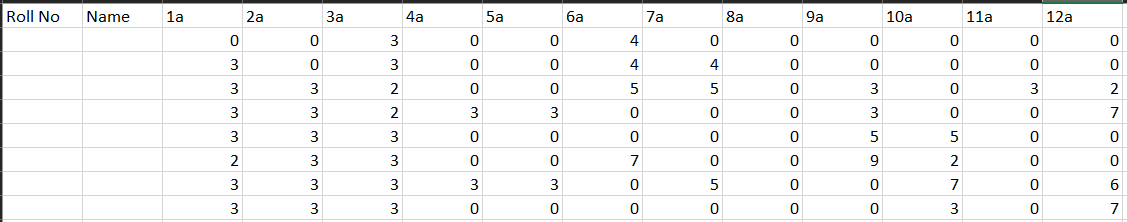
\includegraphics[width=1\textwidth]{Images/prop_sys/csv_output.png}}
% %   \caption{Output CSV File}
% % \end{figure}

% \begin{table}[ht]
%   \centering
%   \small
%   \begin{tabular}{|c|c|c|c|c|c|c|c|c|c|c|c|c|c|}
%   \hline
%   Roll No & Name & 1a & 2a & 3a & 4a & 5a & 6a & 7a & 8a & 9a & 10a & 11a & 12a \\
%   \hline
%    &  & 0 & 0 & 3 & 0 & 0 & 4 & 0 & 0 & 0 & 0 & 0 & 0 \\
%    \hline
%    &  & 3 & 0 & 3 & 0 & 0 & 4 & 4 & 0 & 0 & 0 & 0 & 0 \\
%    \hline
%    &  & 3 & 3 & 2 & 0 & 0 & 5 & 0 & 0 & 3 & 0 & 3 & 2 \\
%    \hline
%    &  & 3 & 3 & 2 & 3 & 3 & 0 & 5 & 5 & 3 & 0 & 0 & 7 \\
%    \hline
%    &  & 3 & 3 & 3 & 0 & 0 & 0 & 0 & 0 & 5 & 5 & 0 & 0 \\
%    \hline
%   \end{tabular}
%   \caption{Output CSV File}
% \end{table}

% \noindent The result is a refined CSV file that has the marks of all students (see a sample of output CSV in Table 3.4). The Roll Numbers and Names can be filled in by the faculty as roll numbers and names were not included in the work. Notably, this CSV file is automatically downloaded through the interface of the application, enabling seamless access to the finalized output on the local system.

% \clearpage

\section{Block Diagram}

\subsection{Overall working of the system}

\noindent Microphone on the device is used to acquire the voice of user. The default voice-to-text in browser will convert it to text. The text is then passed to server for computation. Along with text the primary data of user state is also passed. The server parse the data and modify it to user requirements with set of available functions inside the application. Then invoke Large Language model to respond with JSON instruction of what user meant to perform.\\

\vspace{2 mm}

\noindent LLM respond with JSON is parsed and make sure it mentions available functions only. If JSON response is valid, then it is subjected to execute in Initiative engine we build. It iterate through the JSON and execute each functions and save it values to a collection of objects. If next function requires return value of previous one, then it will check inside that collection. If user is restricted any functions, the entire collection is returned and then asked used for permission. This process is repeated until the iteration ends.

\vspace{2 mm}


\begin{figure}[h!]
    \centering
    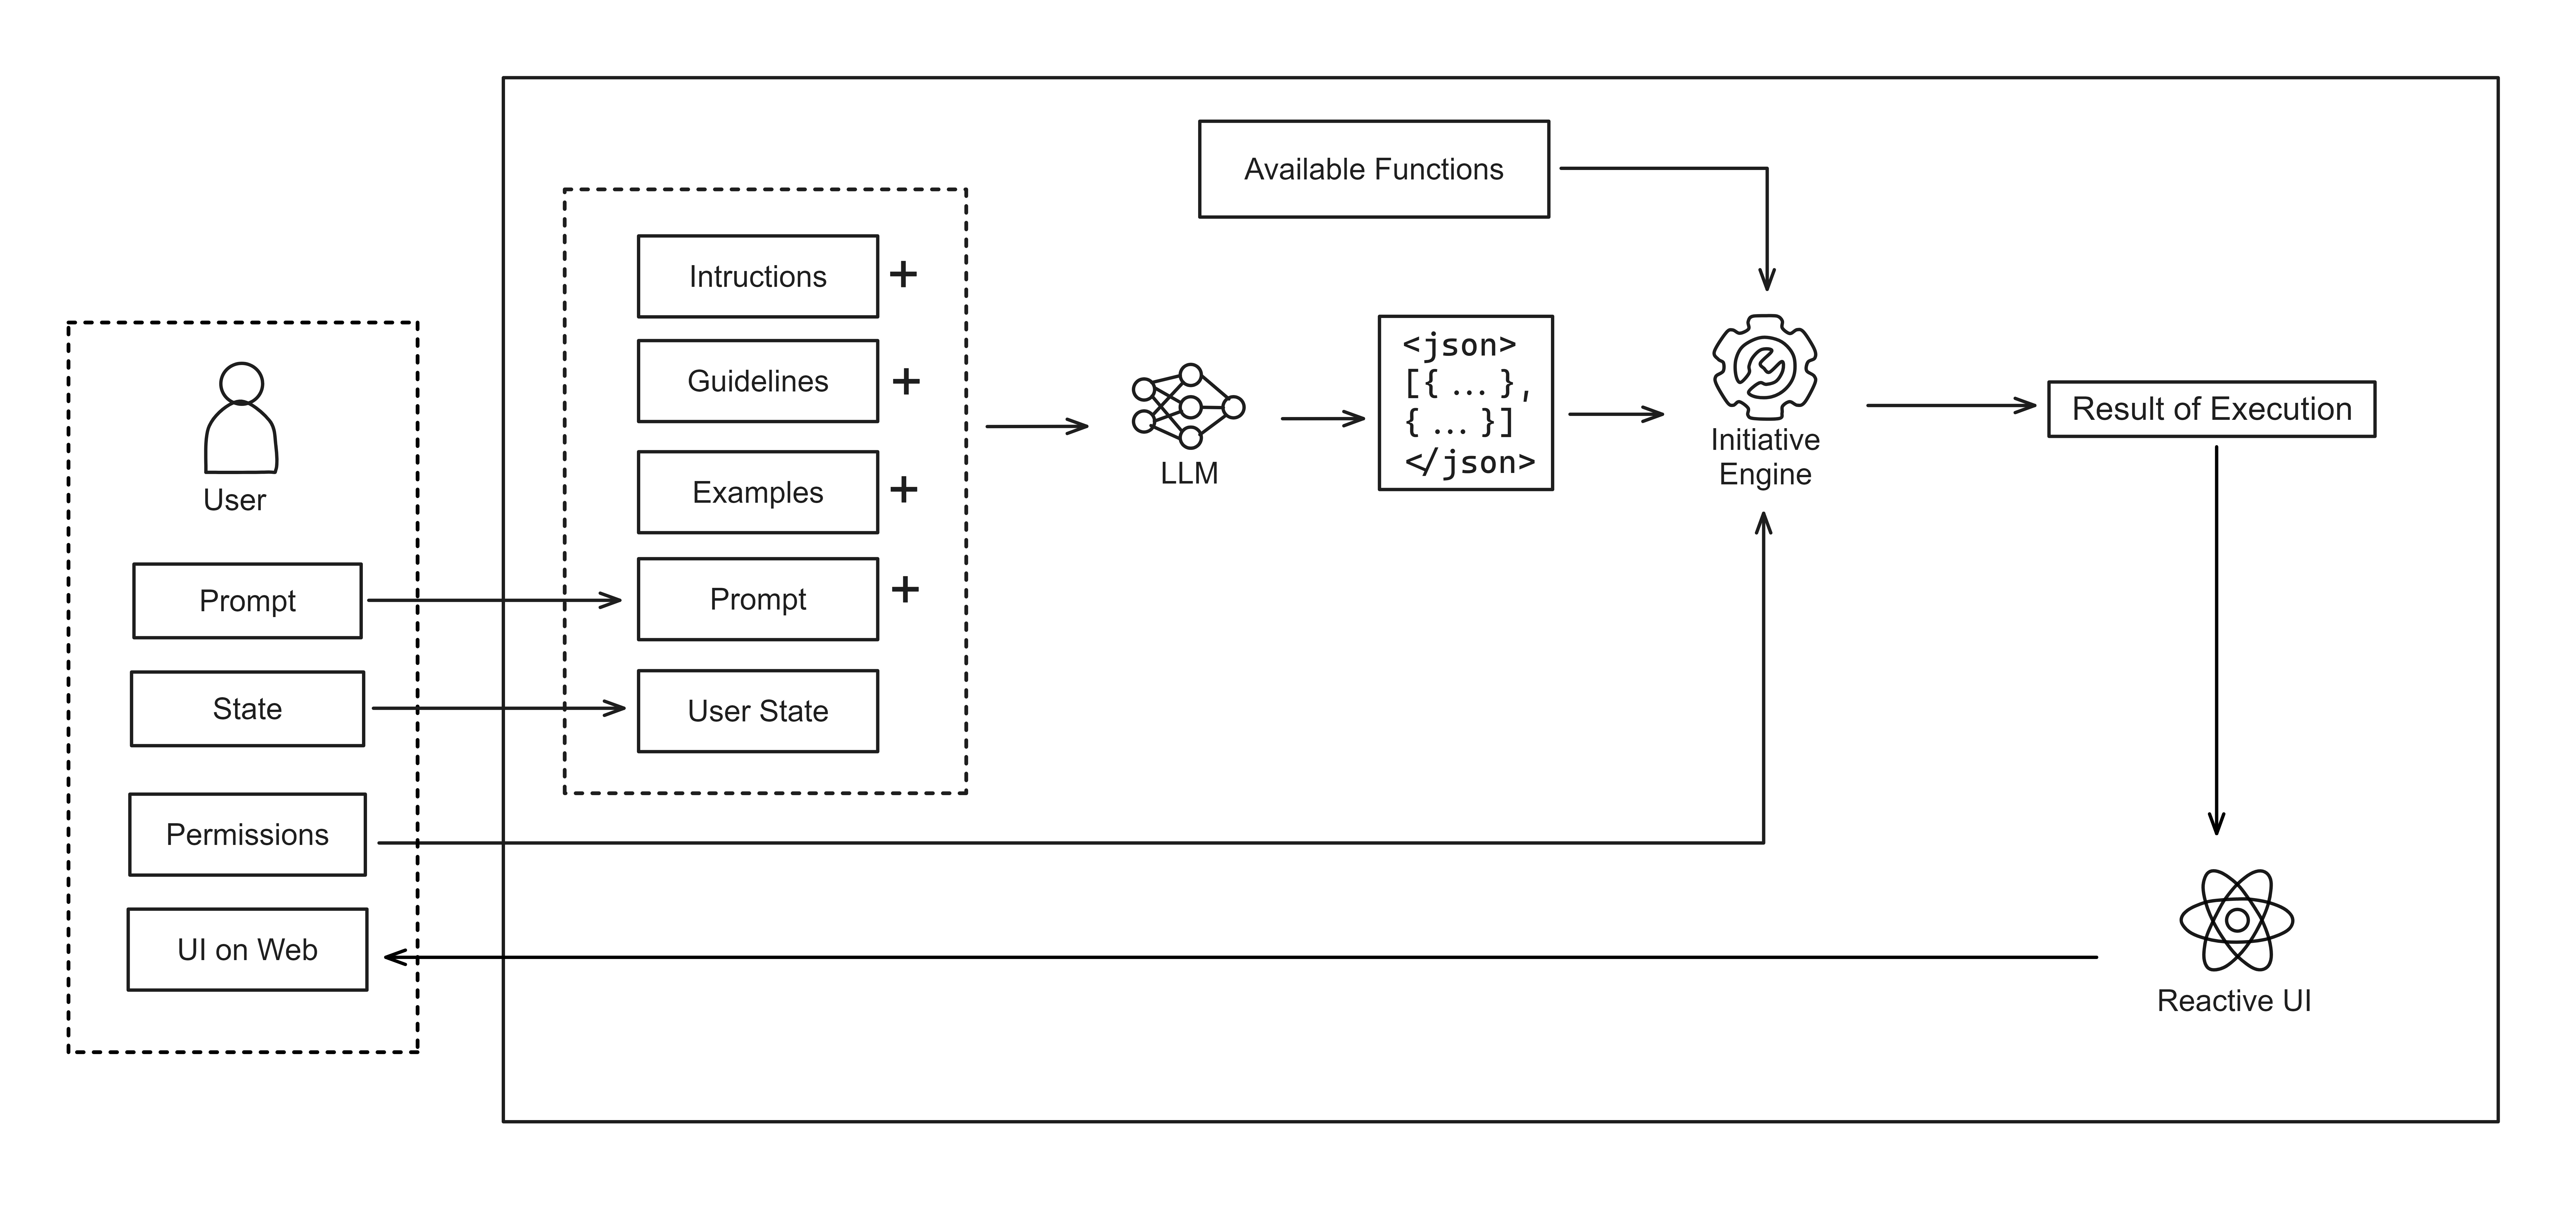
\includegraphics[width=\textwidth]{Images/Block_Diag/Flow_Diagram.png}
    \caption{Working diagram of the proposed system}
\end{figure}

\noindent Finally the collection of function called results are returned along side with the corresponding UI components. Frameworks like NextJs supports server side rendering components instead of rendering ot on client.

\subsection{Data Input}

\noindent In the process of data collection from user as text, the application also collects more user interactions on application. Such as
\begin{itemize} 
    \item User cookies and user data from local storage of browser
    \item User selection on application such as table or contact number
    \item History of recent searches queries 
    \item Results of recent searches
\end{itemize}

\noindent These user data without information about environment is useless to LLM. It can't understand without a proper context about what to do. Thats why LLM need extra data such as

\begin{itemize} 
    \item Instructions to respond in strict JSON format
    \item Guidelines about application specific data
    \item Type definitions of both available functions and response data 
    \item Few short examples for reducing errors
    \item User State and User Input
\end{itemize}

\noindent LLMs can be used with or without fine tuning approaches. Fine-tuning is the process of adjusting the parameters of a pre-trained large language model (LLM) to a specific task or dataset. This involves further training the model on a smaller, domain-specific dataset to enhance its performance and adapt it to the unique requirements of the task at hand. Here application fine tuning help to reduce context window in each request to LLM. 


\begin{figure}[h!]
    \centering
    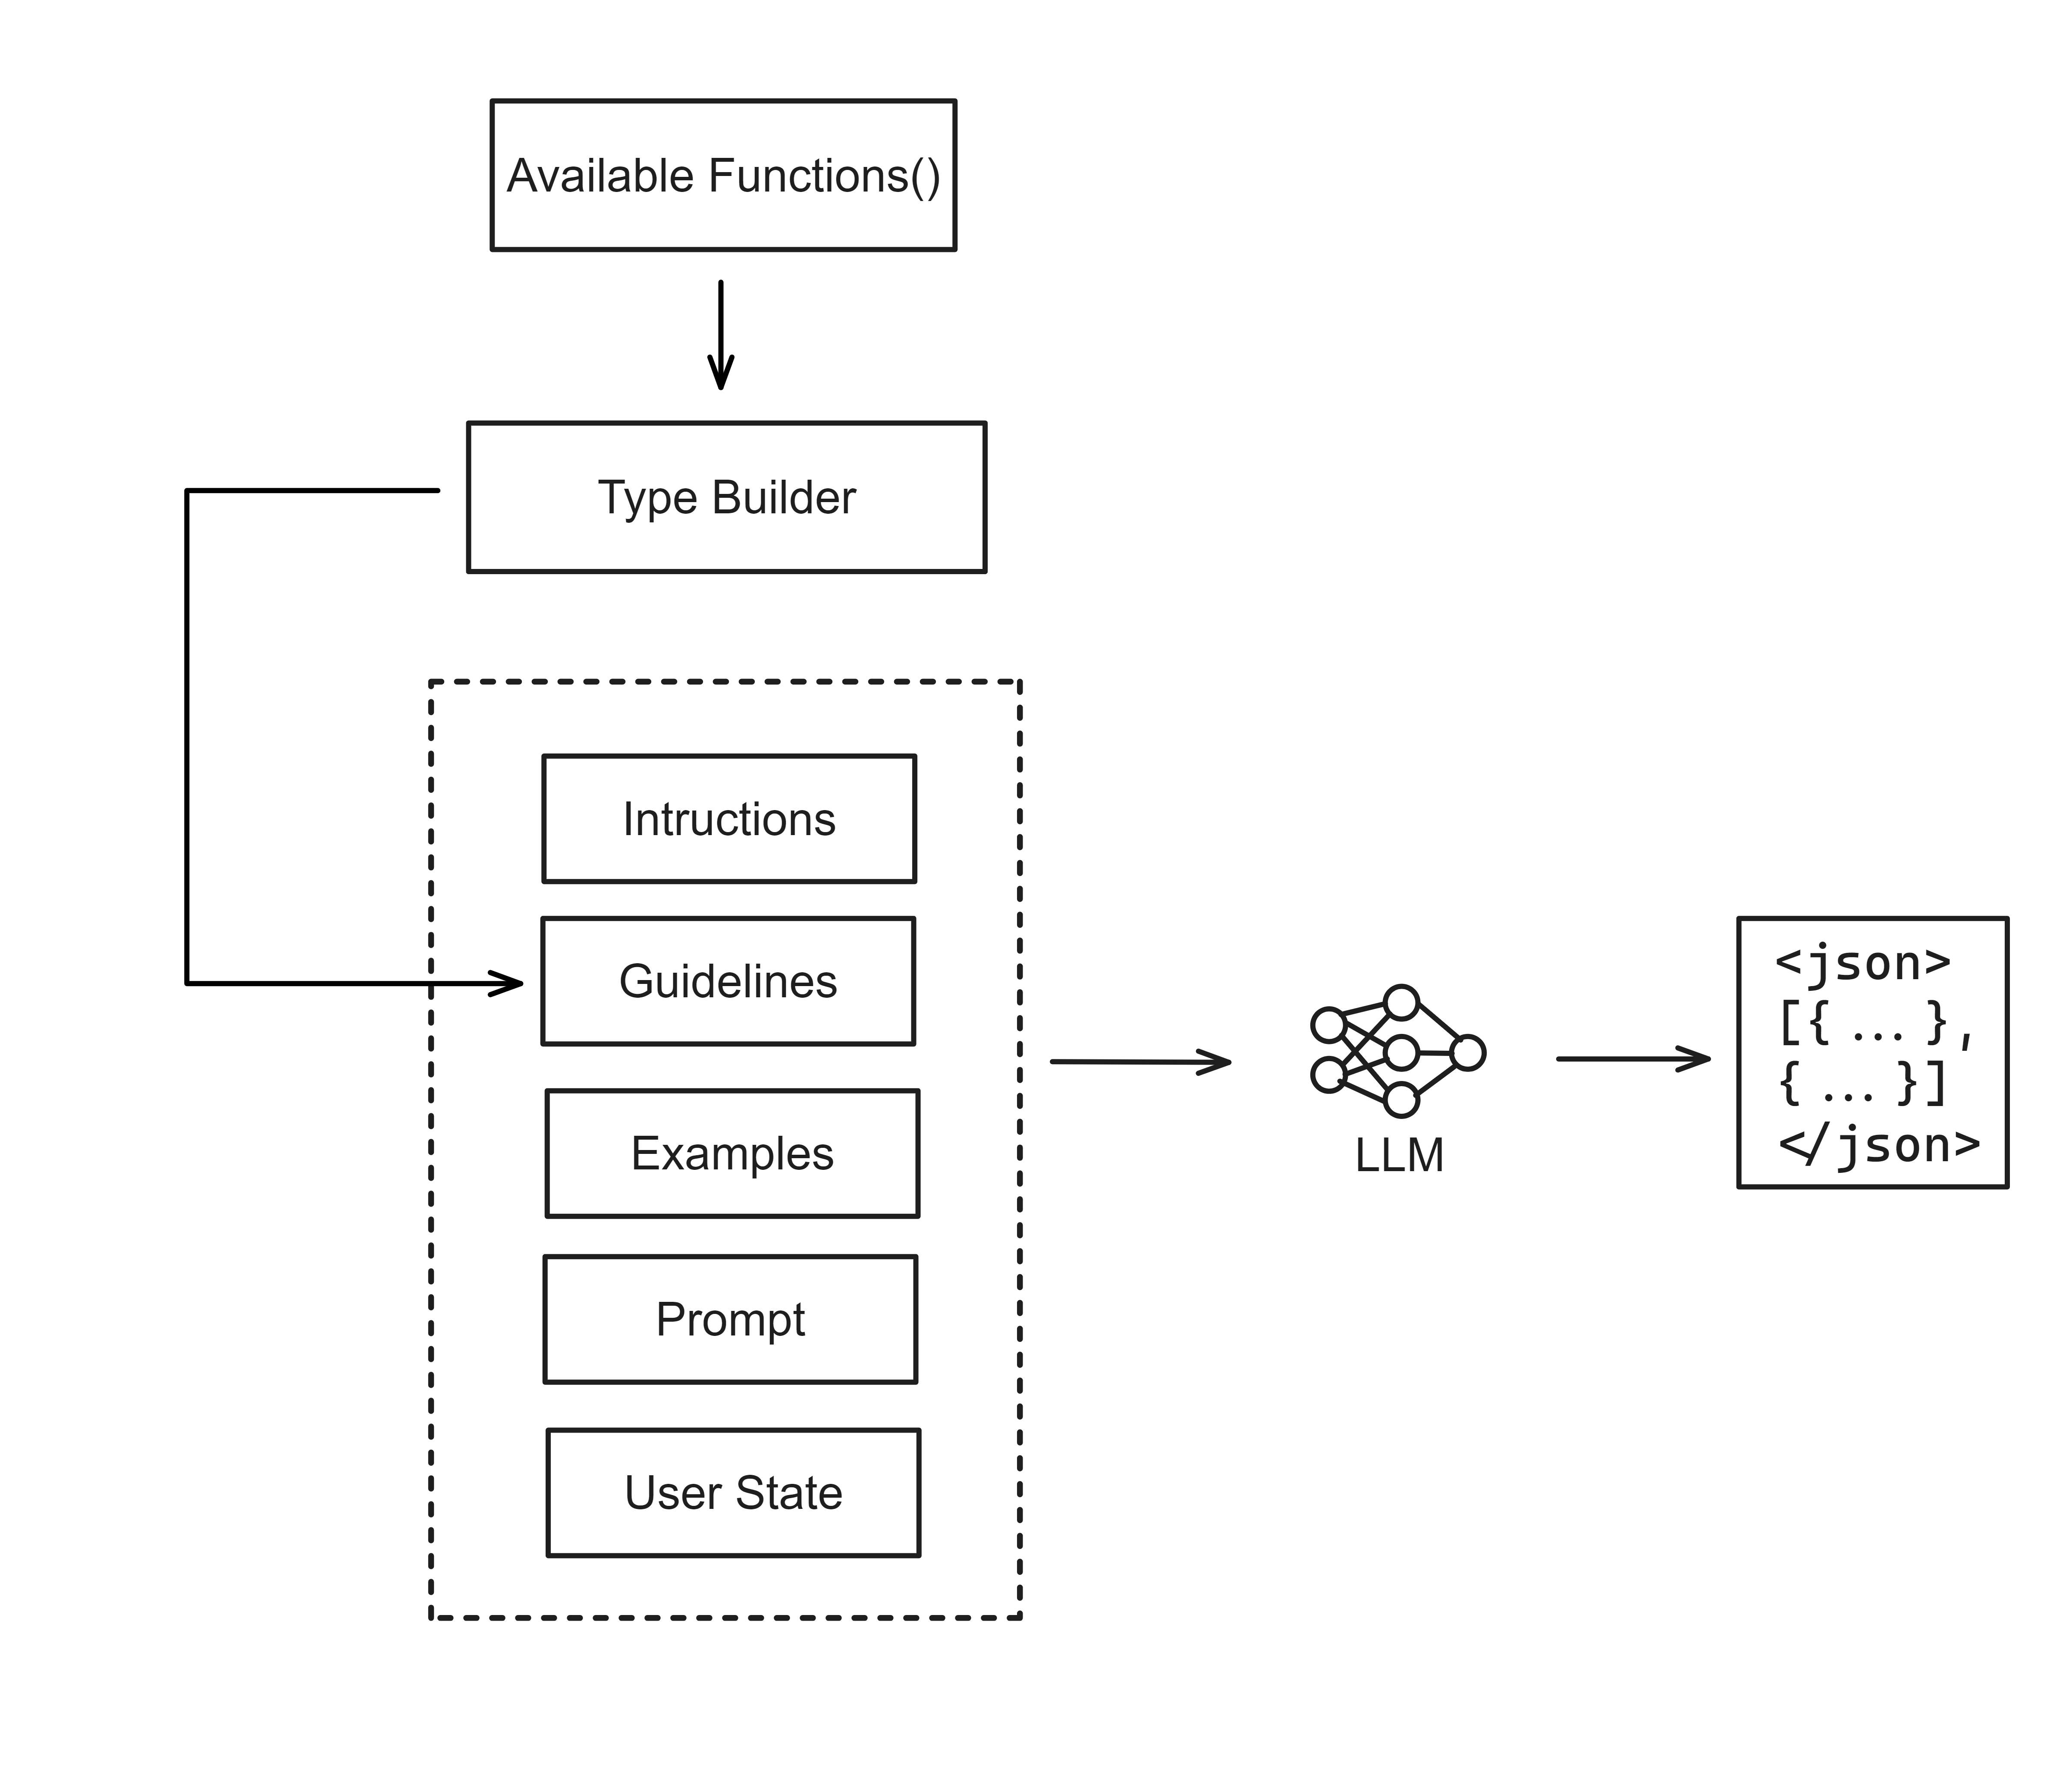
\includegraphics[width=\textwidth]
    {Images/Block_Diag/Without-Fine-Tuning.png}
    \caption{Without Fine Tuning}
\end{figure}
\begin{figure}[h!]
    \centering
    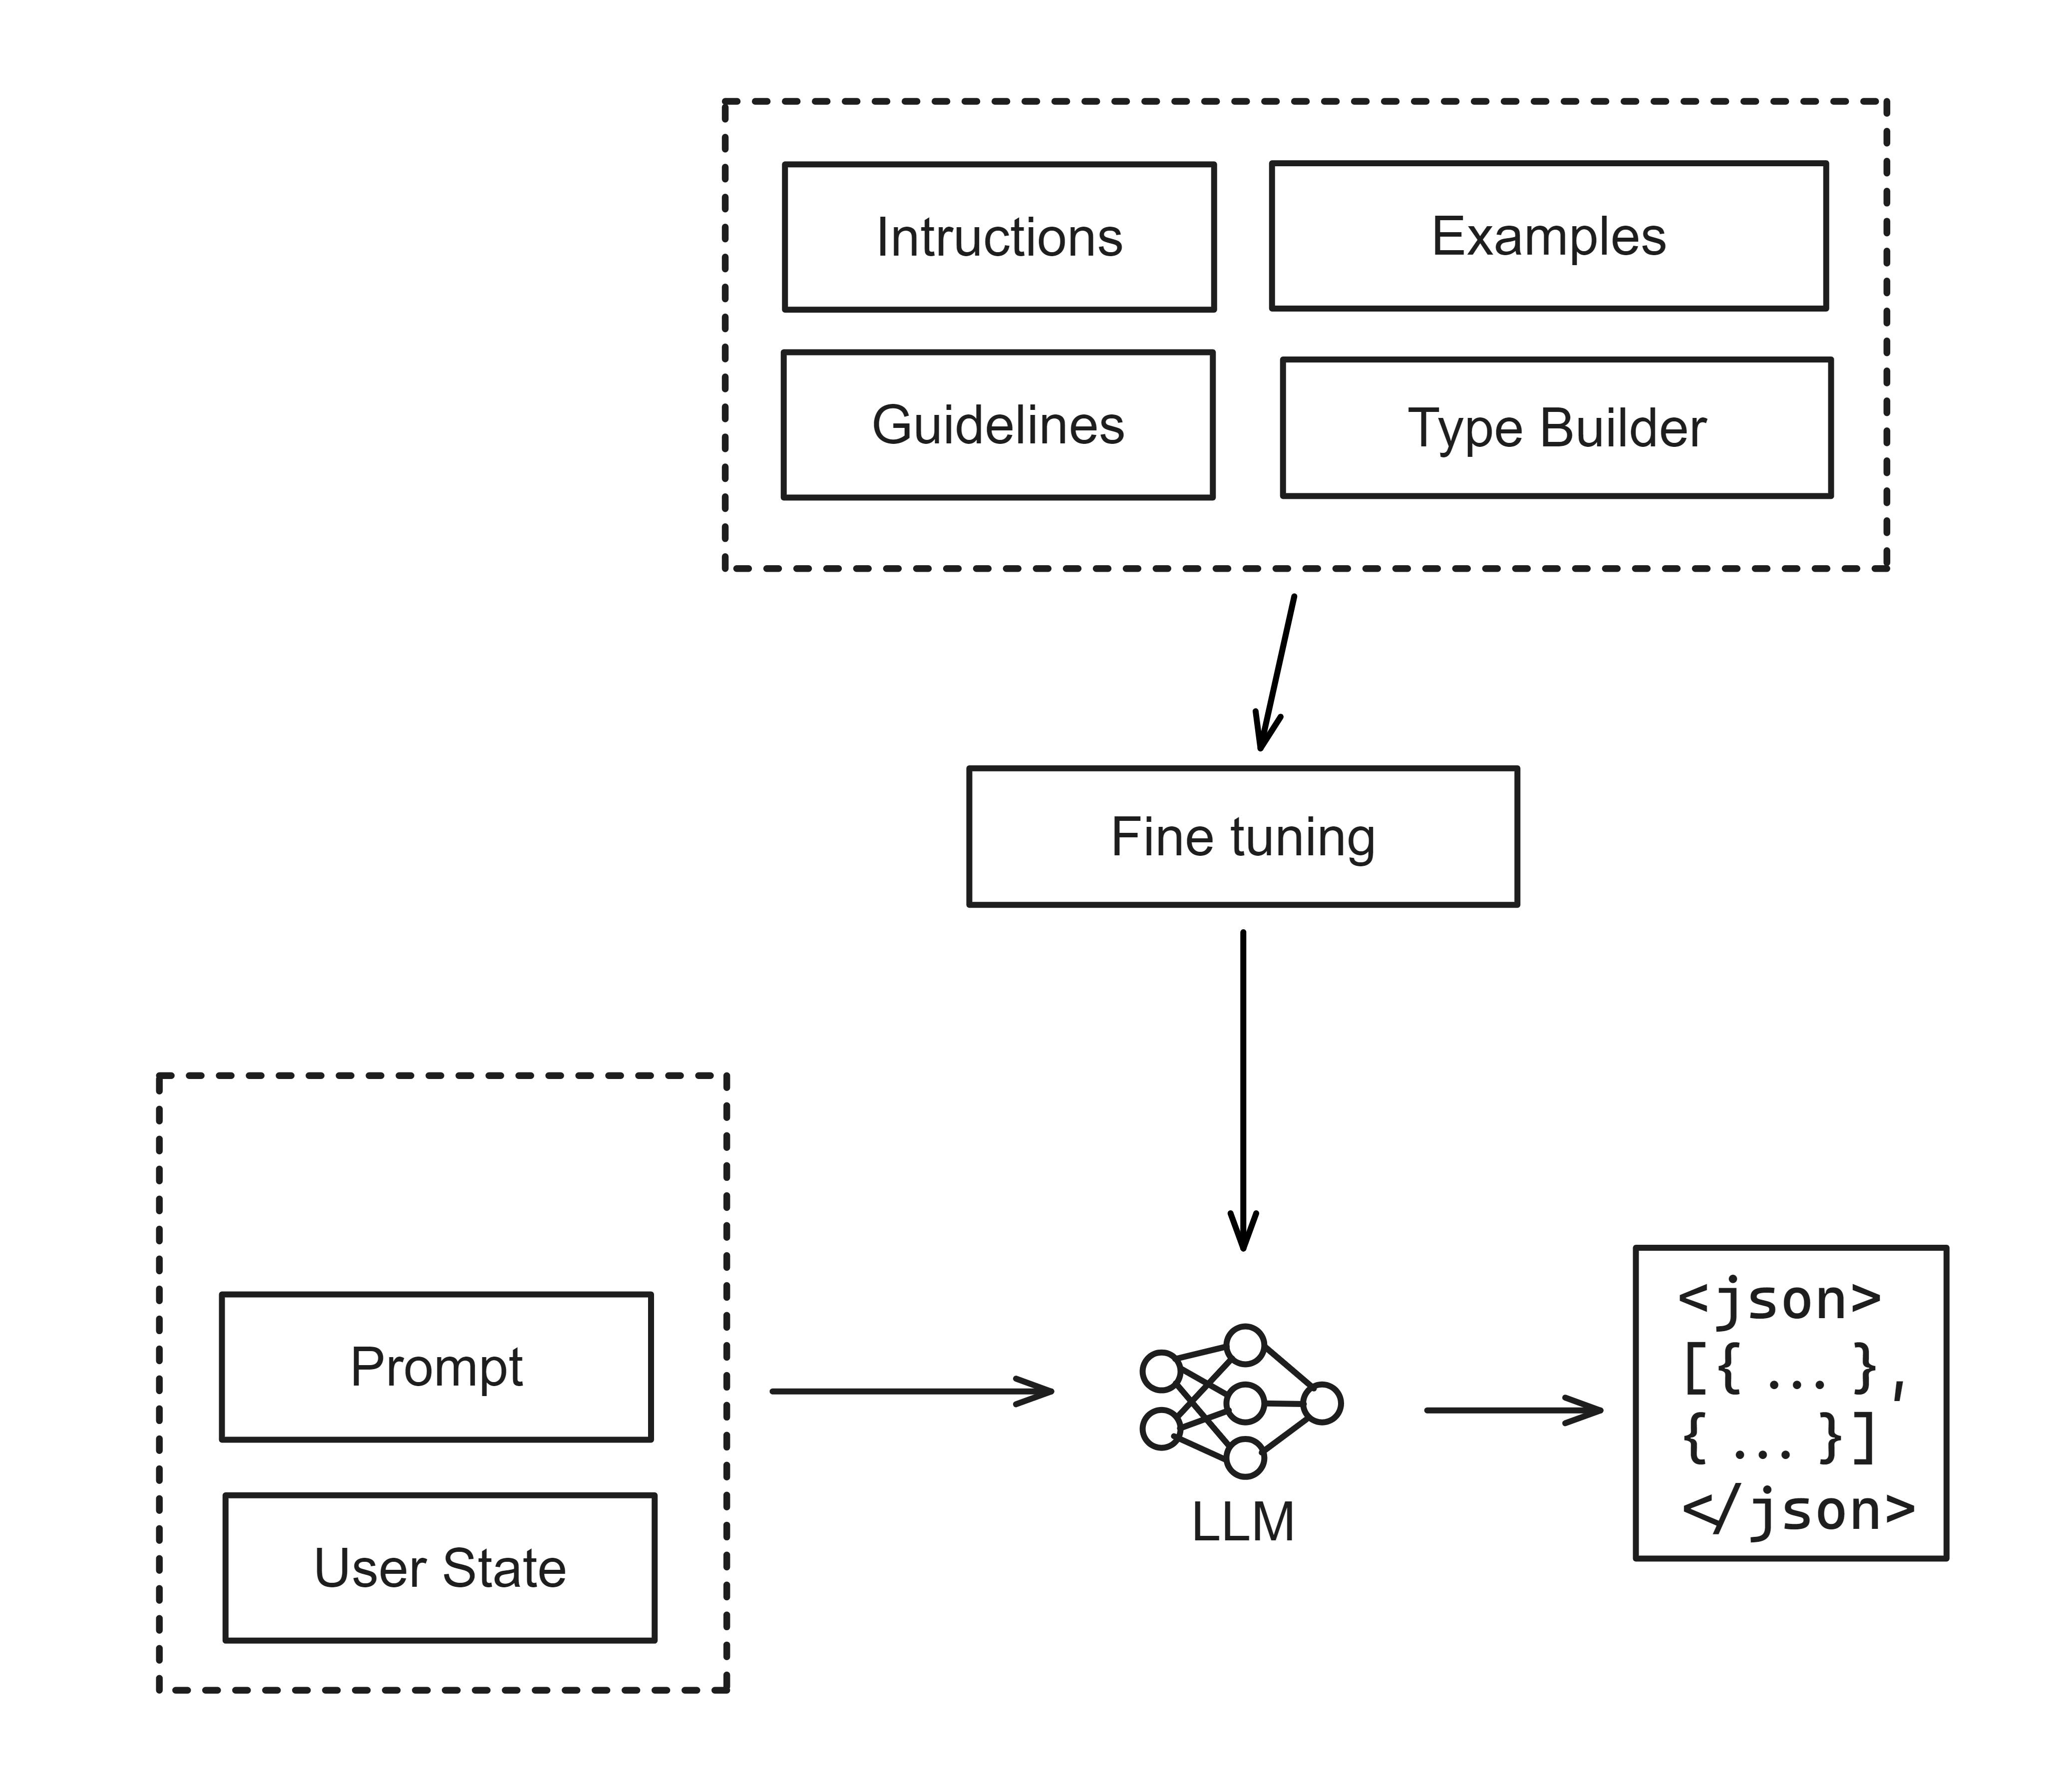
\includegraphics[width=\textwidth]
    {Images/Block_Diag/Fine-Tuning.png}
    \caption{Application Specific Fine Tuning Approach}
\end{figure}

\clearpage

\subsection{Data Pre-processing}

In the process of invoking LLM, a crucial feature to be extracted is type definition of all functions available to this LAM. A TypeScript parser like zod is capable to write the both parser and type definition. The developer of the application need to build their own application specific parser definitions. The Initiative engine will take care of converting that to type definitions to LLM.\\  

The banking applications we built is on TypeScript with LangChain and Zod. LangChain provides great abstractions to build any type of LLM related applications. Zod is used for parsing the input and output data for strict type safety. The custom Initiative we built help to combine all of these and convert LLM to an Action Model.

\begin{figure}[h!]
    \centering
    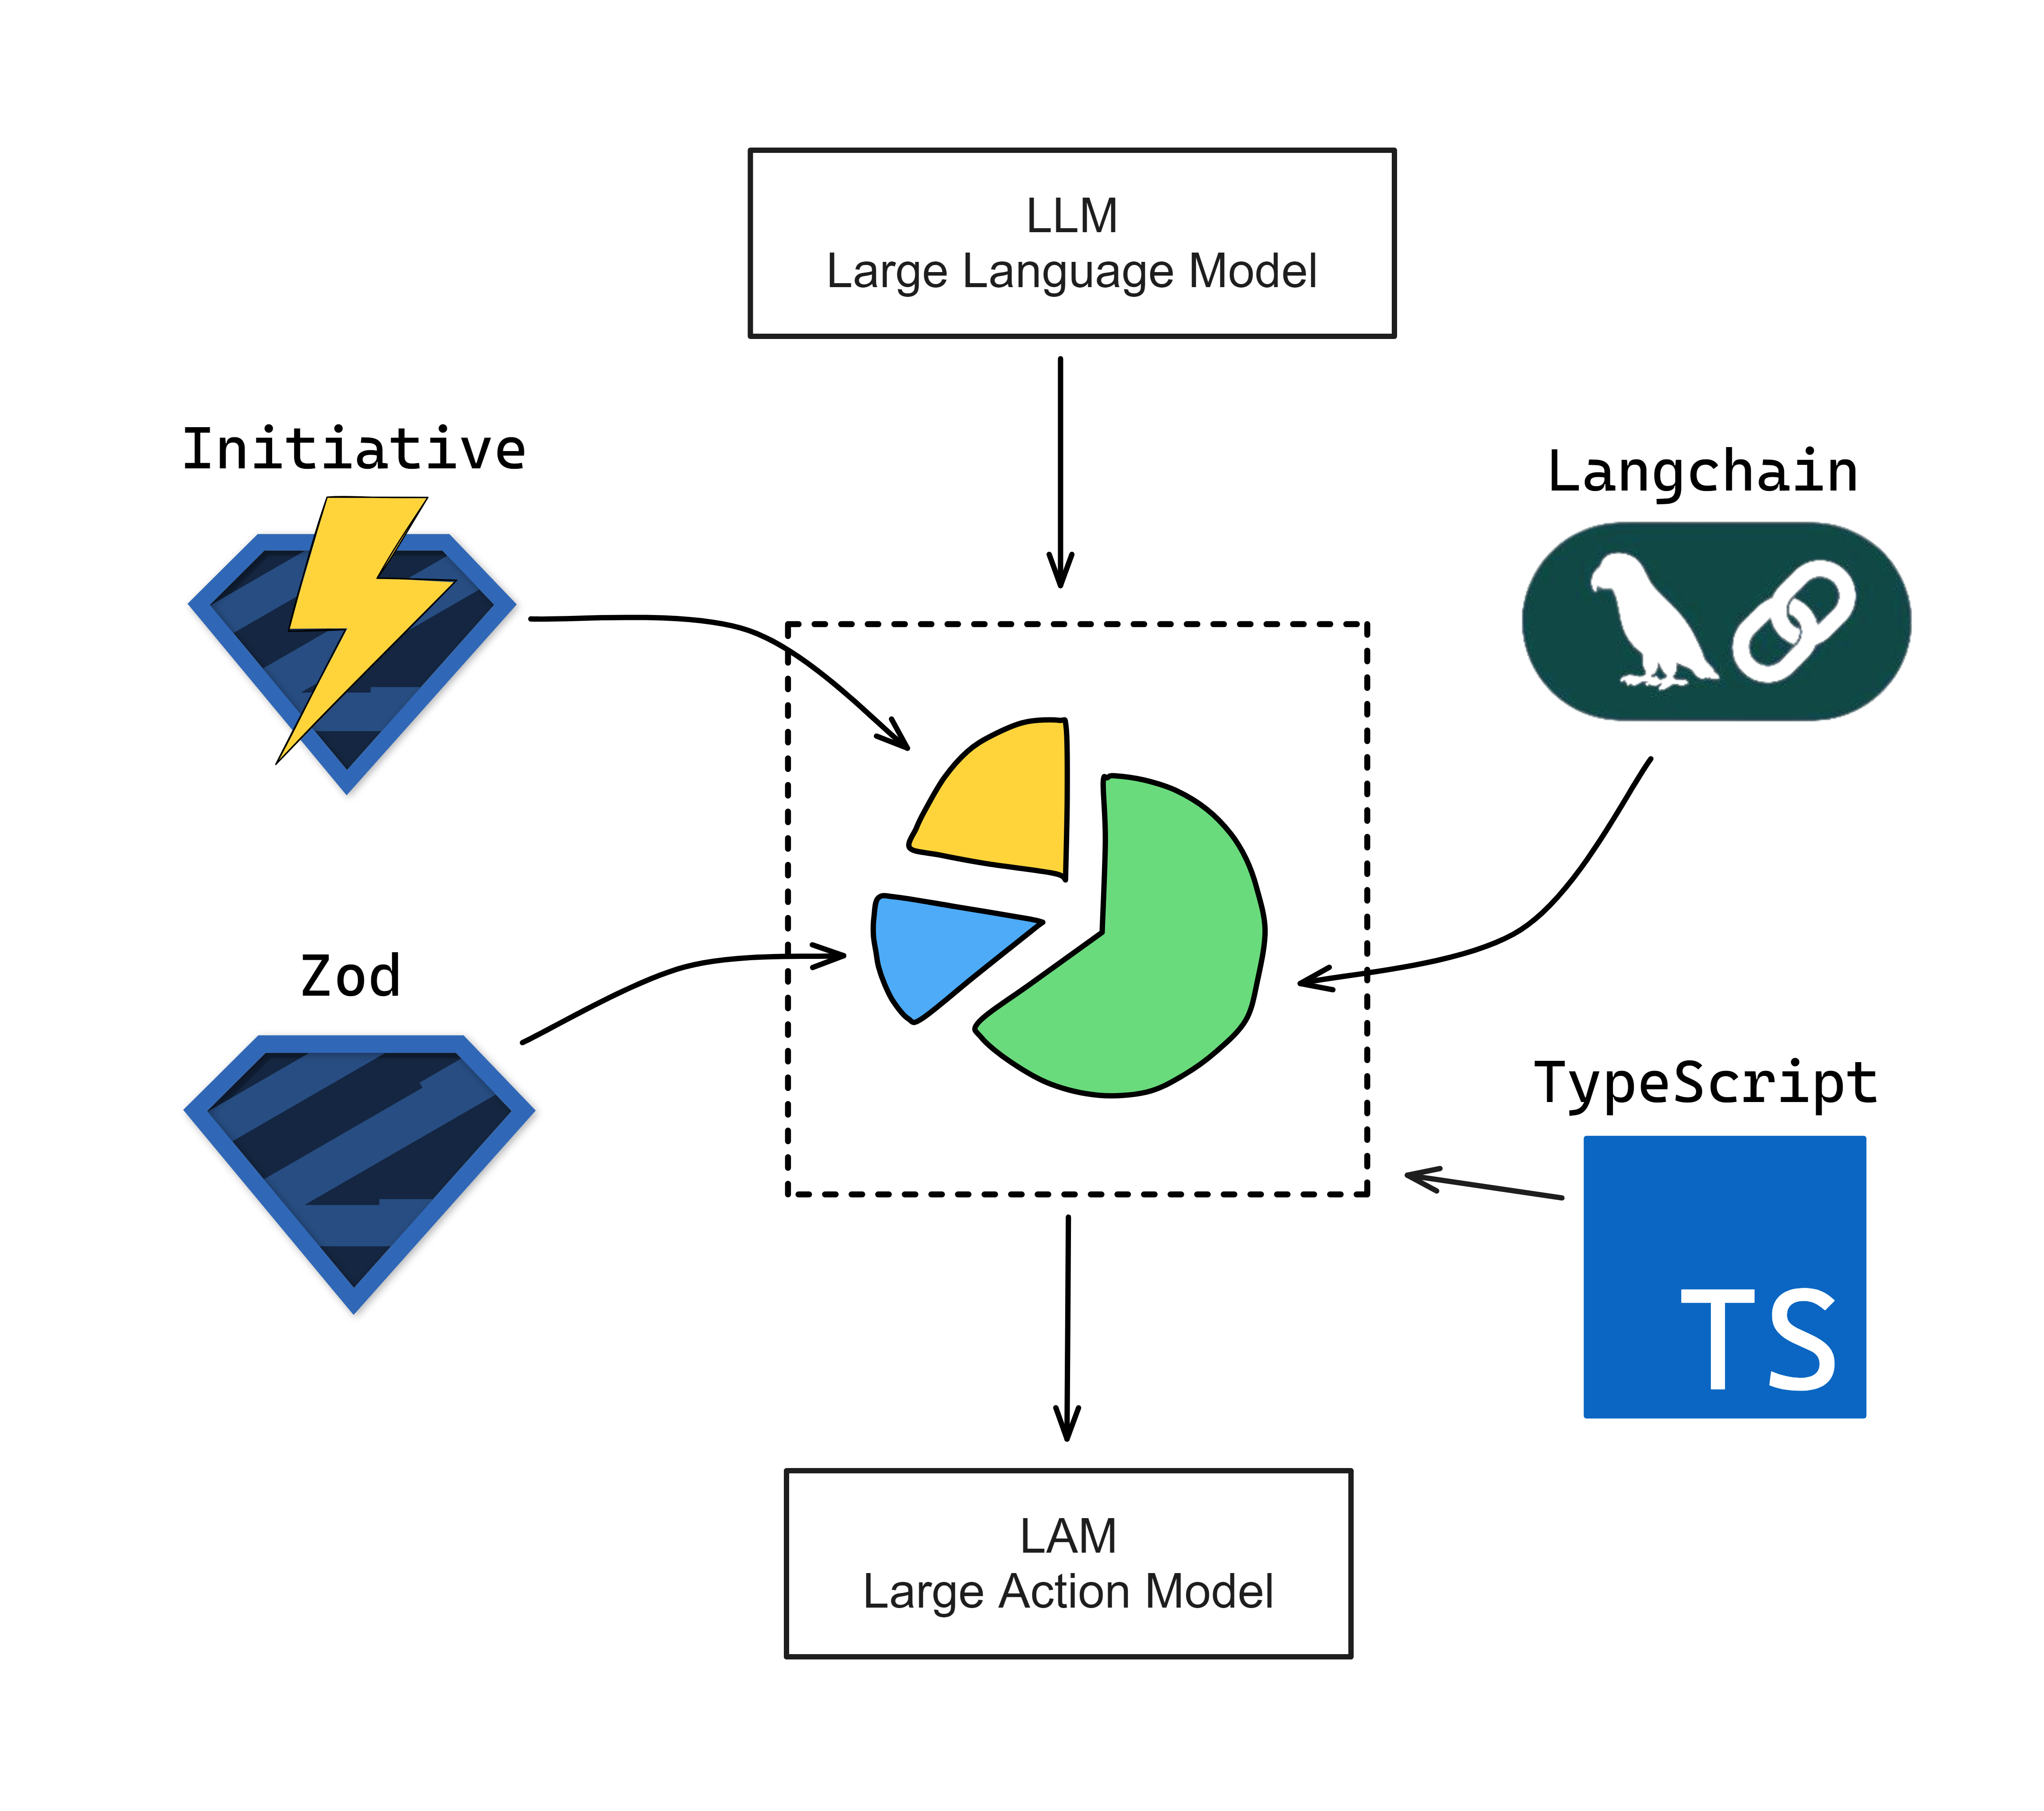
\includegraphics[width=0.8\textwidth]{Images/Block_Diag/LLM-to-LAM.png}
    \caption{LLM to LAM Simple Diagram}
\end{figure}

\clearpage

\subsection{Processing}

\noindent The Action Model Engine is just pure programming without any presence of AI. It is dedicated to run parsed JSON format from LLM. It has access to all available functions. If LLM specifies to run some functions with some parameters, the engine will do that.

\noindent  This system is achieved through a stack and 2 data bucket. The list of function LLM specified to run is stored to stack alongside with the permissions from user. Initial parameters assigned by LLM are stored to Input Bucket. Engine iterate through the stack until stack is empty or permission of any function is denied. In each iteration, it checks the function is available in developer specified list and checks parameters area available in input bucket. If conditions are correctly followed, then it will run the function and save the return value to the Output Bucket. If any condition is failed, the engine returns the entire buckets back to server.

\begin{figure}[h!]
    \centering
    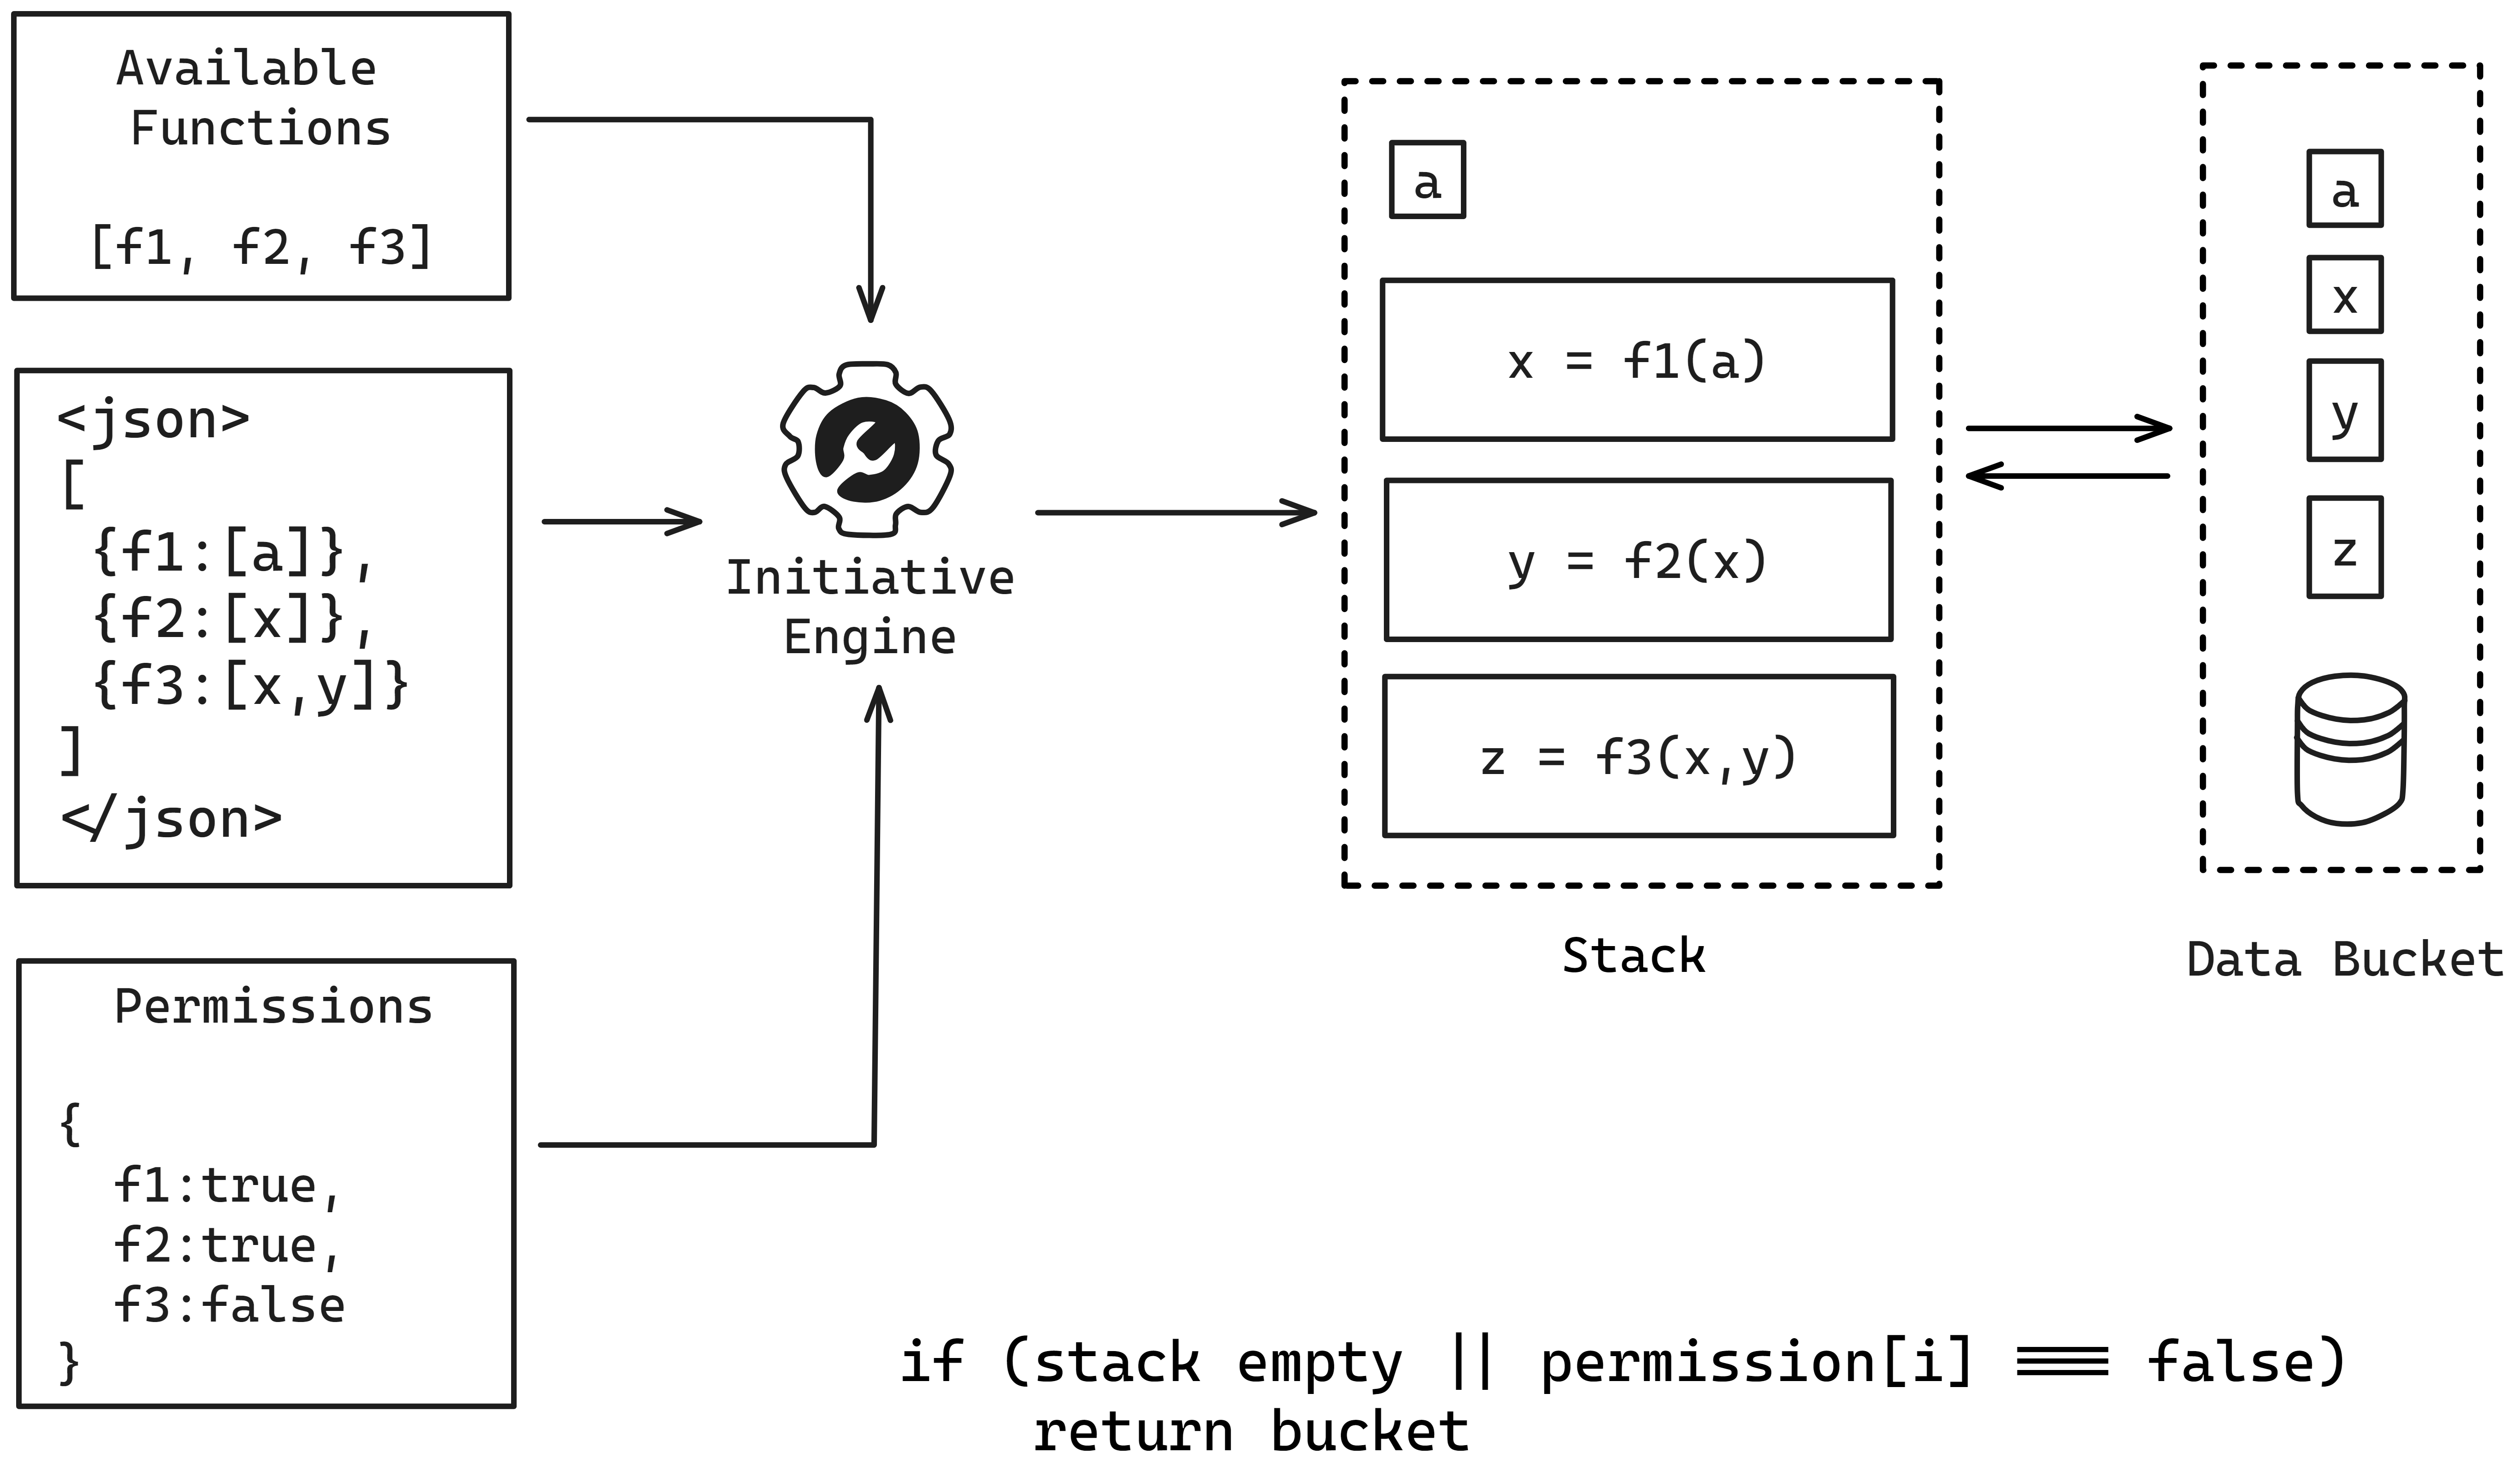
\includegraphics[width=\textwidth]{Images/Block_Diag/engine.png}
    \caption{Action Model Engine (Initiative)}
\end{figure}


\noindent This methodology ensures the efficiency and accuracy of the system in the extraction of data and function calling, making it a reliable and valuable tool developers to build their own action models on top any LLMs.

\subsection{Post-processing}

\noindent After obtaining the result in the form of a list of return values, the server return them to client alongside with UI components of each data. With help of modern meta-frameworks technologies we can choose server-side rendering or client-side rendering. Server side rendering help to reduce security vulnerabilities because data is completely on control of server and client side browser only gets rendered HTML, CSS.

\noindent If server returns data back to client due to permission error, then user is again asked to allow the access of functions to continue executing. The engine will re-execute and returns with updated state.

\begin{figure}[h!]
    \centering
    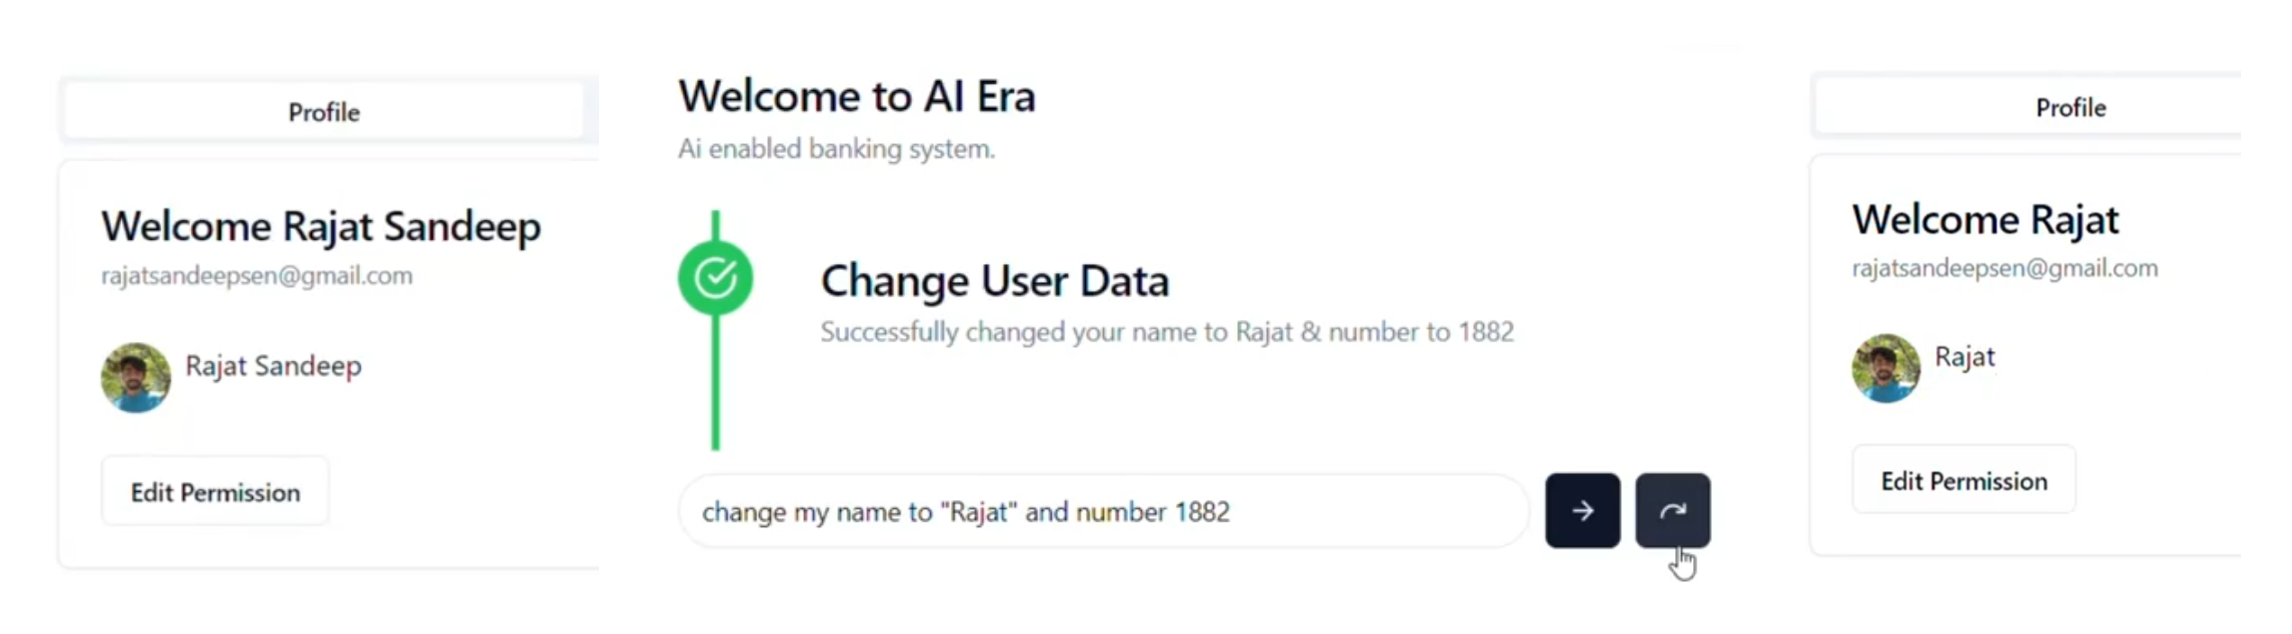
\includegraphics[width=\textwidth]{Images/Block_Diag/invoke-one-function.png}
    \caption{User asked to alter the details (Invoked single function)}
\end{figure}


\begin{figure}[h!]
    \centering
    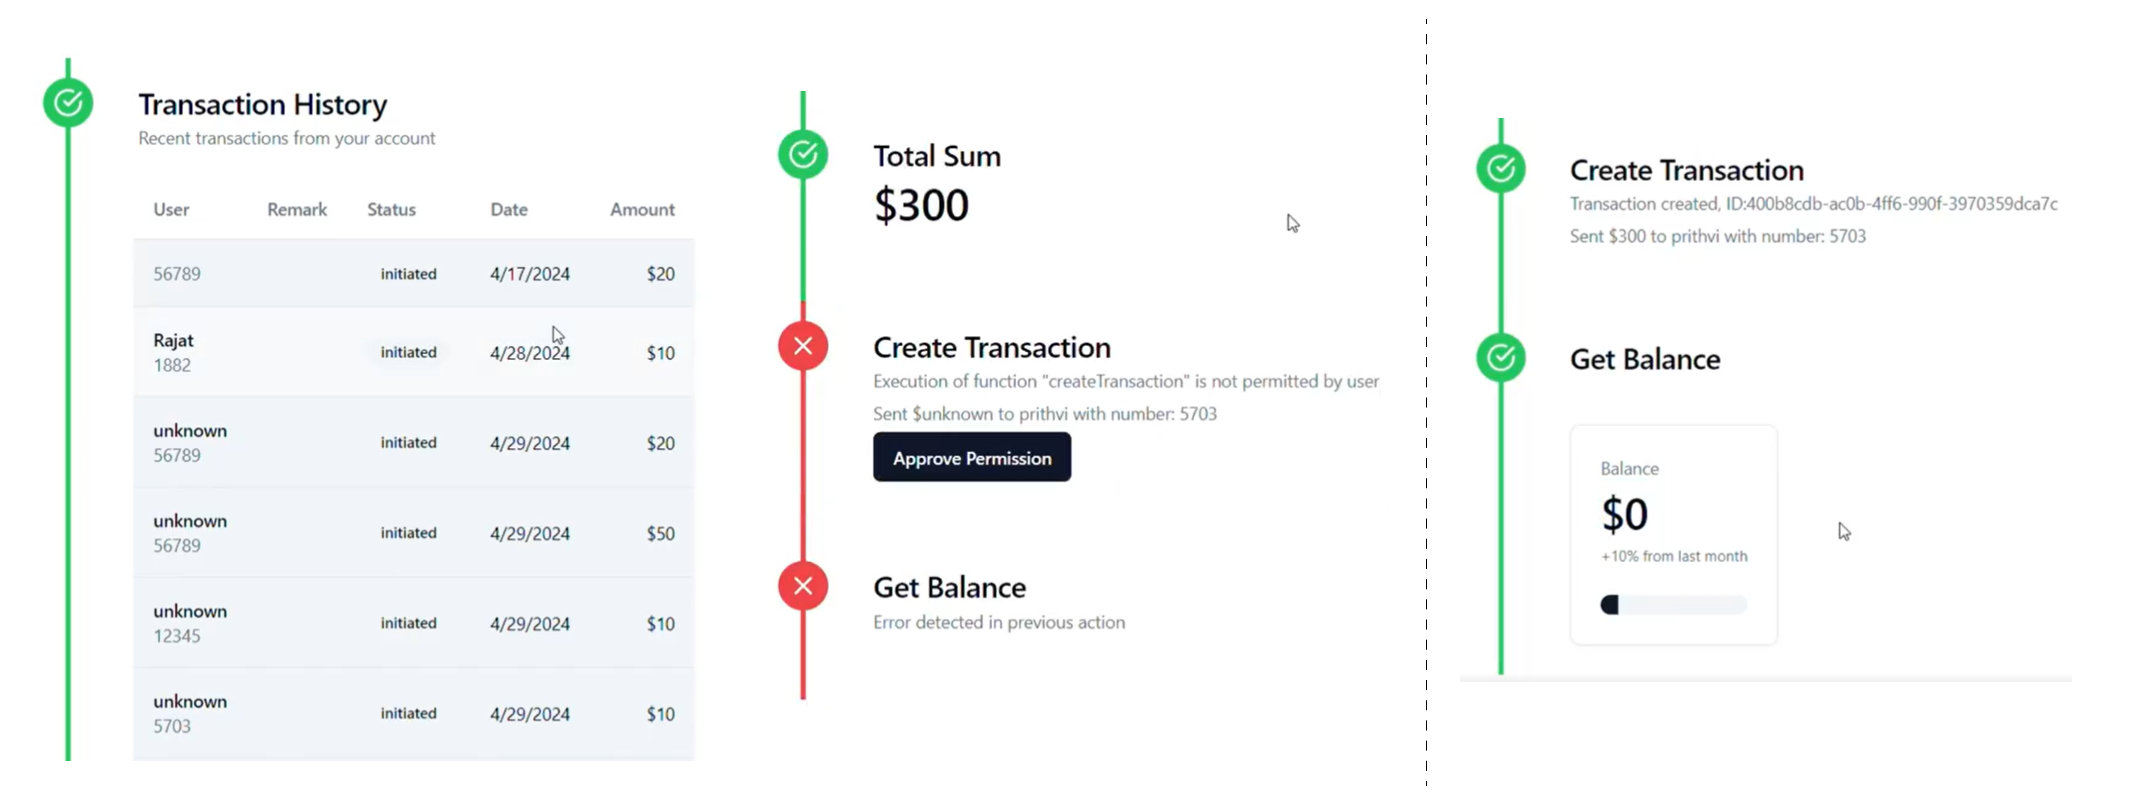
\includegraphics[width=\textwidth]{Images/Block_Diag/transaction-example.png}
    \caption{User asked multiple requirements (and denied one last function)}
\end{figure}


\section{Summary}

% \vspace{0.5mm}

\noindent
The proposed system which is discussed in detail performs very efficiently in comparison with existing systems. The computation time of the proposed system varies from application to application and inference provider used for responding with Intelligence. The proposed system is capable of achieving an average time of 2-6 seconds for the computation.

\clearpage